
% 开题报告
% \begin{figure}[htb] % use float package if you want it here
%     \centering
%     
\includegraphics{hello}
%     \caption[基于利益相关者的人-水关系分析框架]{图4.1. 基于利益相关者的人-水关系分析框架。(a.)基于社会交换理论的人际关系互动,人与人之间通过付出代价与获得报酬来维持关系。(b.)“虚假相依”,利益相关者不期为人-水关系付出代价,仅按照自己意图行事以获得报酬。(c.)非对称相依,利益相关者愿意在维持自身意图的情况下为人-水关系付出代价,以期获得更多的报酬。(d.)“反应性相依”,利益相关者付出代价并仅依赖于人-水关系获得报酬。
%     该框架不同于前人从不同人-水关系主题或不同区域的角度出发所作的分类,这里基于利益相关者提出的人-水关系分析框架仅考虑了人(利益相关者)在人-水关系中的行事意图,因此针对不同类型、不同结果的人-水关系都具有分析参考意义。}\label{ch2:fig:reaction}
% \end{figure}

% % 开题报告
% 社会交换理论强调关系中存在报酬和代价,而人际交往的关系就可以通过这种报酬和代价的交换来完成[67]。在人际关系互动中,参与互动的两方在互动中投入代价并获得报酬,如果两者都不期望在关系中付出代价或获得报酬,那么这种关系的密切程度自然不及互相付出并获得报酬的关系。
% 通过将人-水关系视为一种人与水的交往过程,我们可以参考基于社会交换理论的“依存关系”,根据利益相关者付出报酬和获得代价的不同路径来分析人-水关系。
% 由于水文系统总是按照自己的意愿(客观规律)行事,所以人-水关系的互动模式主要取决于人如何付出代价并获得报酬:(1)当利益相关者完全不为水文系统付出代价以期获得报酬时,相互作用的双方均按照自己的意愿行事,人与水文系统仍然存在交互,但这种交互并不基于人类主动去“维护关系”,所以被称为“虚假相依”(图3b)。(2)当利益相关者不仅愿意为自身意图付出代价,还愿意为干预水文系统付出代价,以期两者共同给予自身更多报酬时,这种关系可被视为“非对称相依”(图3c )。(3)当利益相关者仅靠对水文系统的关系中付出代价才能获得报酬时,这种关系可以被视为“反应性相依”(图3d)。


人地关系地域系统是人类活动与地理环境相互作用、形成的具有地域特征的系统\cite{tan2021},流域是一个完整的地理单元,所有的利益相关者都与流域的某些水文要素或过程有关。
在流域尺度下需要考虑的利益相关者应做出取舍,因为人水关系是人地关系的一种,具有多重性、异时相关性、异地相关性、人的主动性、动态性和多重决定性的特征\cite{fang2004},很难通过显式表达穷尽其与水圈要素过程的全部关系,需要忽略冗余部分并找到流域系统的主导因素。
因此,本研究的原则是把握“人水关系是指导流域研究的宏观整体性概念”,识别并针对主导流域人水关系的利益相关者及其与水圈要素、过程的关联状态,分析不同阶段间的变化。

流域系统是一个典型的社会-生态系统,其关键特征是复杂自适应性(见图\ref{ch2:fig:concepts}),人水关系不是所有利益相关者关系的简单加和(机械系统观),而是系统内外所有人水关系产生的动态平衡(复杂适应性系统观)。
不同的流域演变阶段,流域特征可以由中央管理者自上而下控制(控制系统),也可以由尺度更小的利益相关者自下而上涌现(自组织系统),因此主导流域人水关系的利益相关者状态并不确定。
本研究对人水关系演变过程的机制分析,重点便是这种自上而下的驱动力和自下而上的驱动力如何改变利益相关者与水圈要素、过程的关系。

基于上述理论与概念,本研究对“流域系统人-水关系”给出如下便于研究的定义:

{\kai~在流域尺度下,主导复杂人水系统“自然-社会二元循环结构”的利益相关者基于自身利益,通过决策与地球表层系统中水圈的要素、过程相连接的状态。}

\begin{figure}[htb] % use float package if you want it here
    \centering
    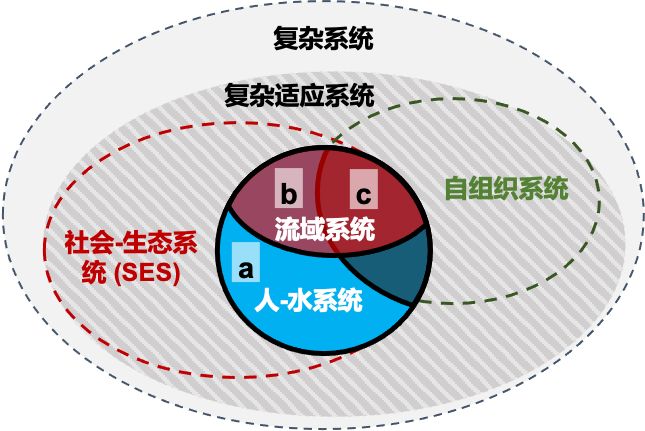
\includegraphics[width=0.6\textwidth]{img/ch2/ch2_concepts.png}
    \caption[流域系统作为社会-生态系统的概念图式]{流域系统作为社会-生态系统的概念图式}\label{ch2:fig:concepts}
\end{figure}


\begin{figure}[htb]
    \centering
    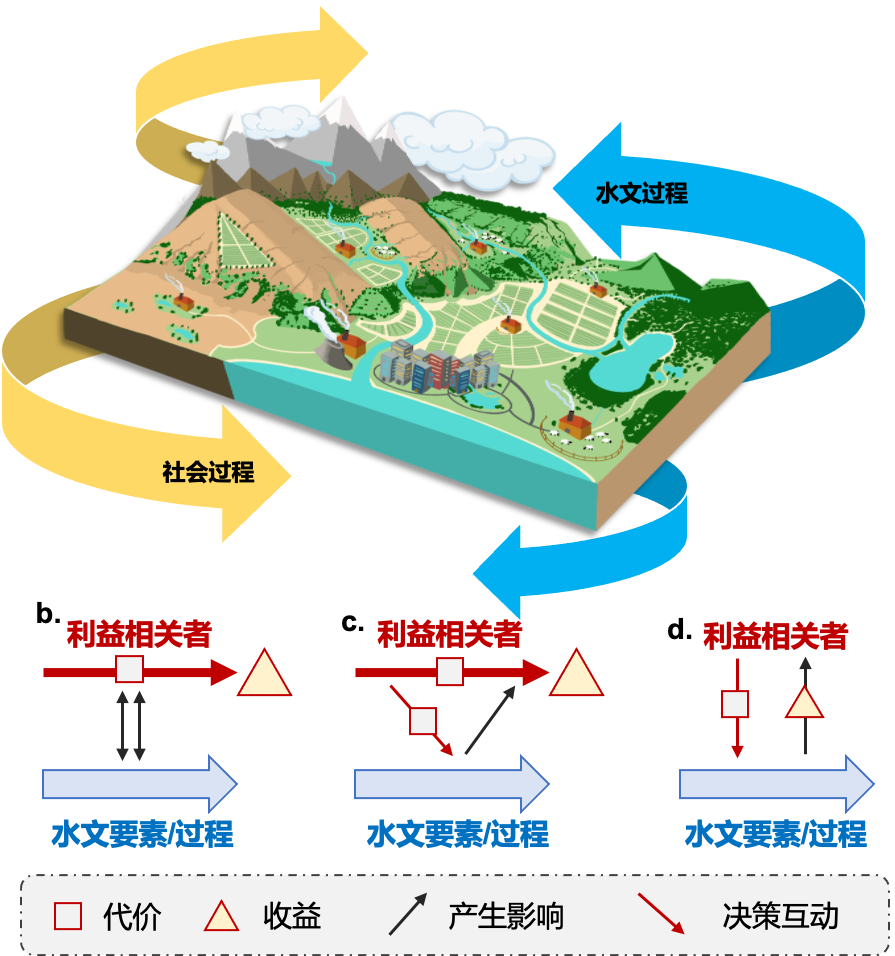
\includegraphics[width=0.6\textwidth]{img/ch2/ch2_interactions.png}
    \caption{利益相关者与水文系统的连接状态}\label{ch2:fig:interactions}
\end{figure}
